\begin{frame}{Positional Encoding}

  \begin{itemize}
    \item[$\blacktriangleright$] Transformers lack sequence order awareness.
    \item[$\blacktriangleright$] \textbf{Positional encodings} are added to input embeddings to provide information about token positions.
    \item[$\blacktriangleright$] \textbf{Sinusoidal encoding:}
  \end{itemize}
  
  \vspace{0.8em}
  
  \begin{align*}
    PE(pos, 2i) &= \sin\left(\frac{pos}{10000^{\frac{2i}{d_{\text{model}}}}}\right) \\
    PE(pos, 2i+1) &= \cos\left(\frac{pos}{10000^{\frac{2i}{d_{\text{model}}}}}\right)
  \end{align*}

\end{frame}

\begin{frame}{Positional Encodings}
  \centering
  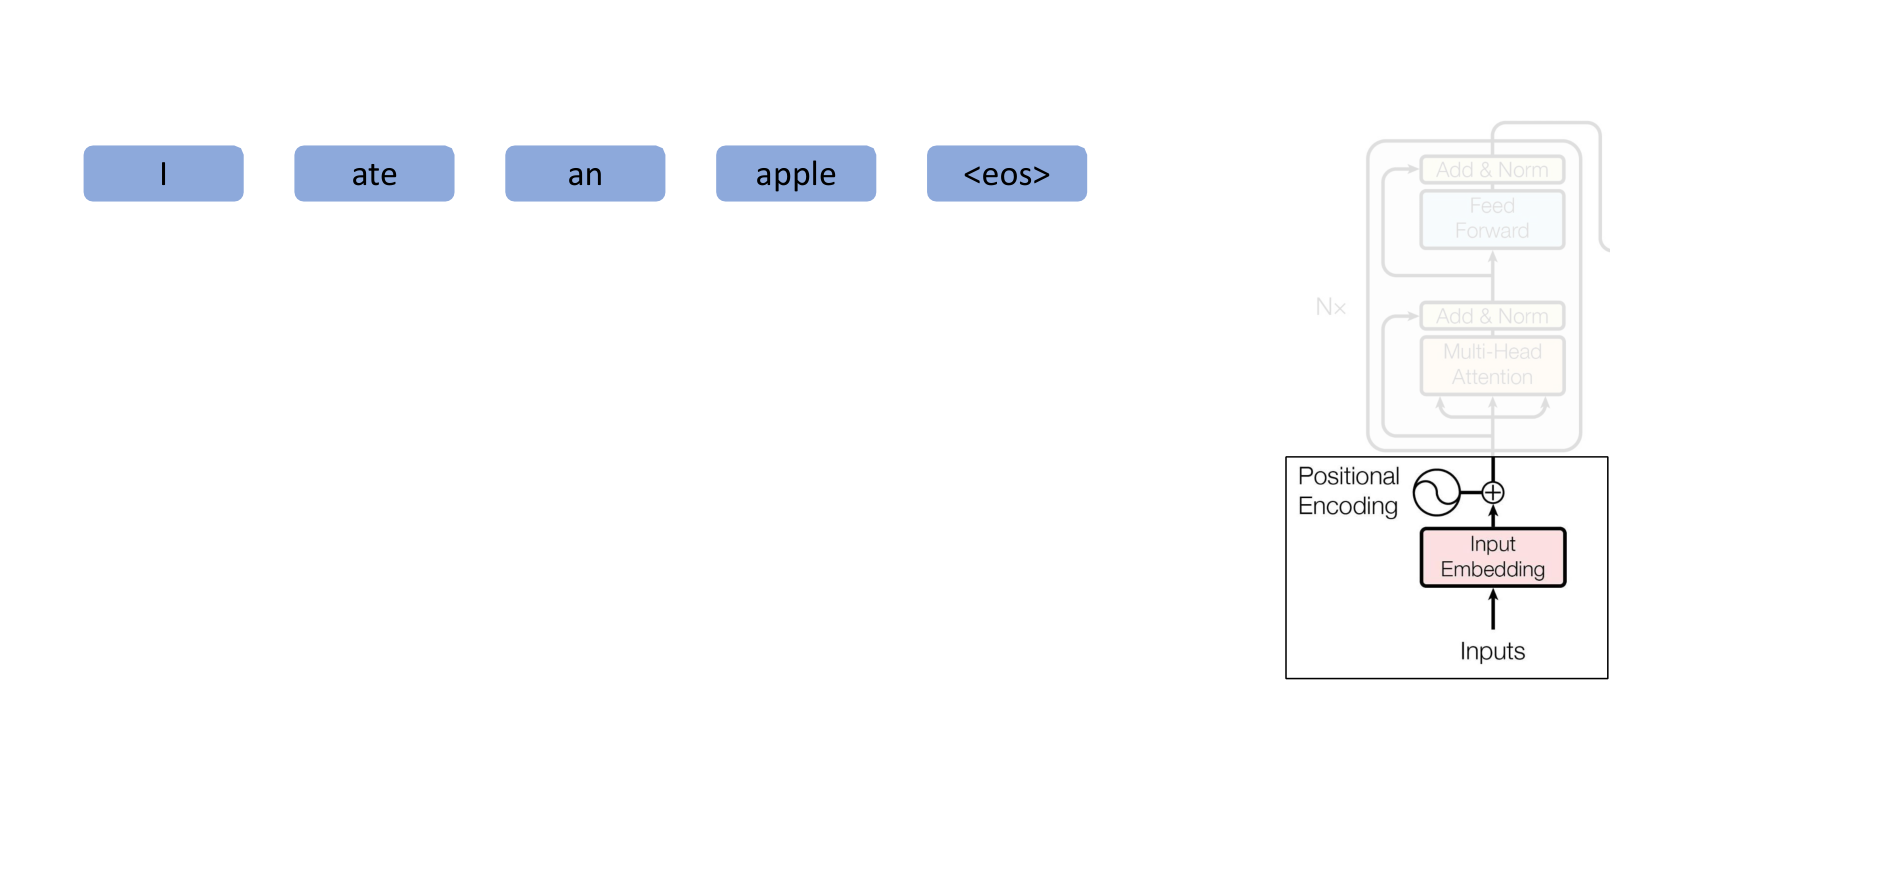
\includegraphics[width=\linewidth,height=0.75\paperheight,keepaspectratio]{images/introduction-to-transformers/transformer_input_embedding_highlight_tokens_sequence.png}

  {\scriptsize Source: CMU 11-785, Lecture 19 ``Transformers,'' Spring 2024, slide 13.}
\end{frame}

\begin{frame}{Positional Encodings}
  \centering
  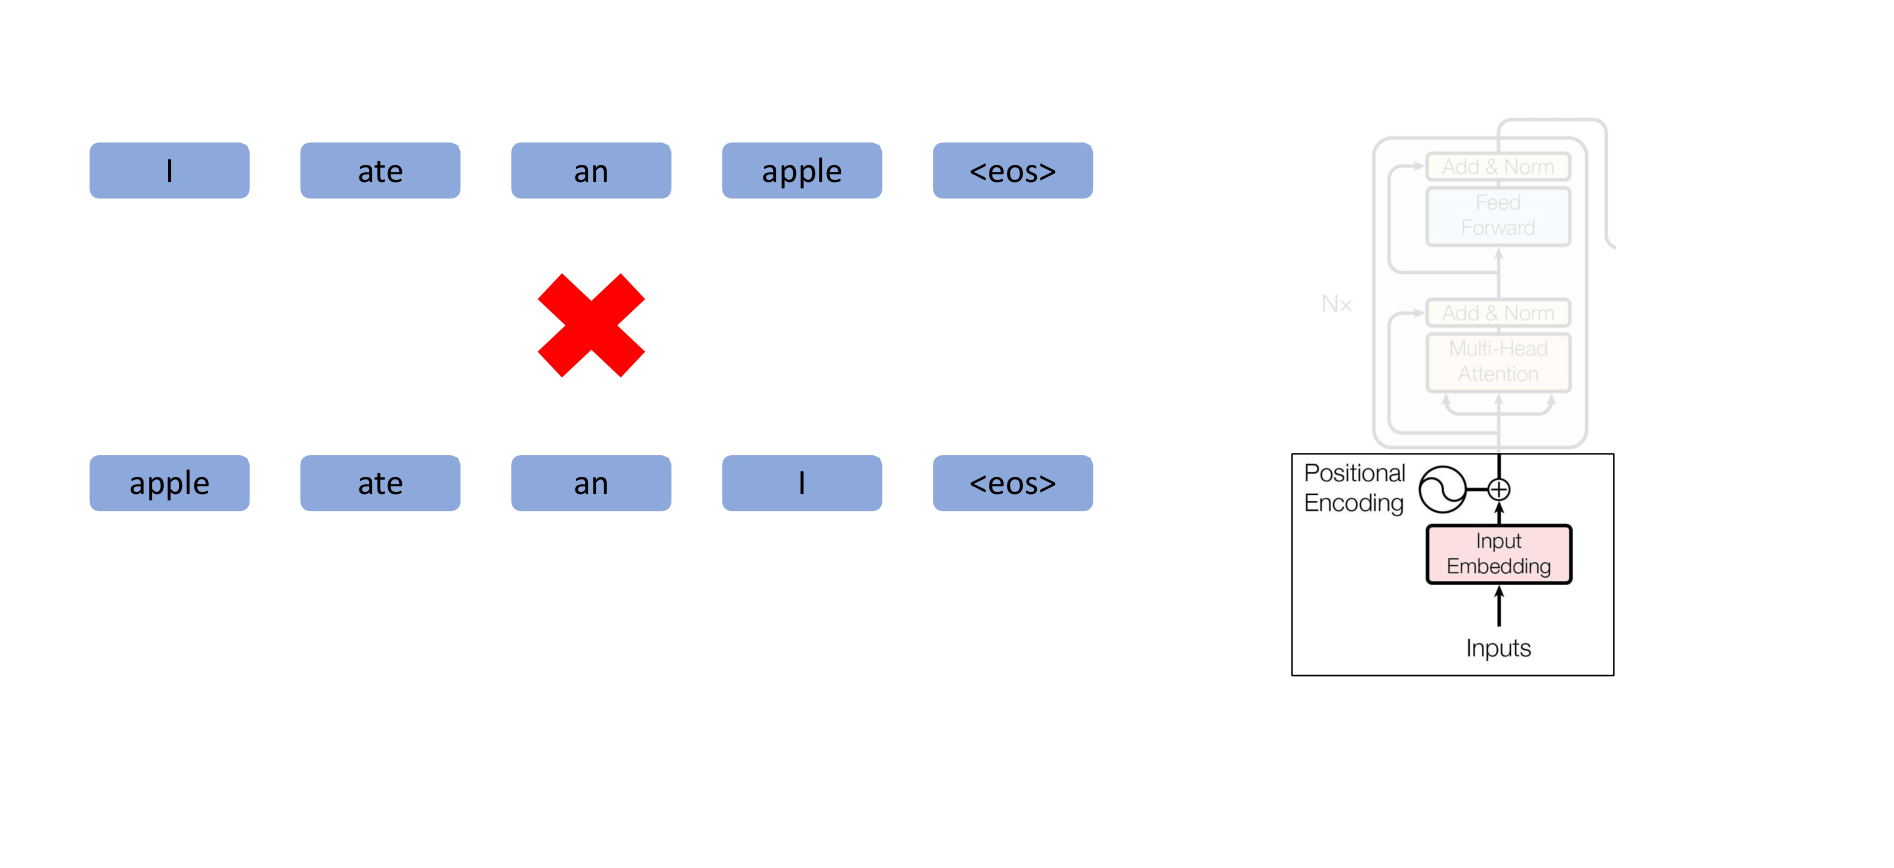
\includegraphics[width=\linewidth,height=0.75\paperheight,keepaspectratio]{images/introduction-to-transformers/transformer_word_order_matters_scrambled_tokens.png}

  {\scriptsize Source: CMU 11-785, Lecture 19 ``Transformers,'' Spring 2024, slide 14.}
\end{frame}

\begin{frame}{Position Encodings}
  \begin{columns}
    \begin{column}{0.6\textwidth}
      \textbf{Requirements for Positional Encodings???}
    \end{column}
    \begin{column}{0.4\textwidth}
      \centering
      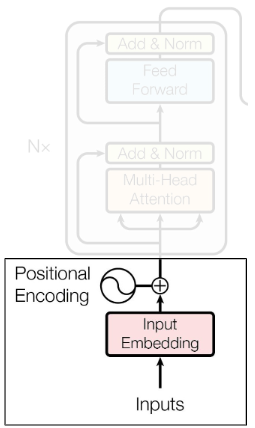
\includegraphics[width=0.5\paperwidth,height=0.5\paperheight,keepaspectratio]{images/introduction-to-transformers/transformer_input_embedding_block_diagram.png}

      {\scriptsize Source: CMU 11-785, Lecture 19, Spring 2024.}
    \end{column}
  \end{columns}
\end{frame}

\begin{frame}{Position Encodings}
  \begin{columns}
    \begin{column}{0.6\textwidth}
      \textbf{Requirements for Positional Encodings}
      \begin{itemize}
        \item Some representation of time? (like \texttt{seq2seq}?)
        \item Should be unique for each position -- not cyclic
      \end{itemize} 
    \end{column}
    \begin{column}{0.4\textwidth}
      \centering
      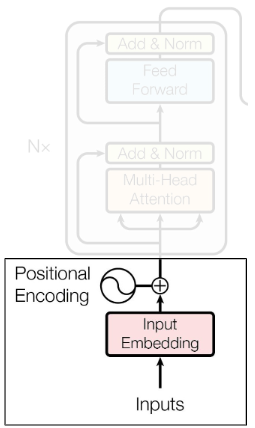
\includegraphics[width=0.5\paperwidth,height=0.5\paperheight,keepaspectratio]{images/introduction-to-transformers/transformer_input_embedding_block_diagram.png}

      {\scriptsize Source: CMU 11-785, Lecture 19, Spring 2024.}
    \end{column}
  \end{columns}
\end{frame}

\begin{frame}{Position Encodings}
  \begin{columns}
    \begin{column}{0.6\textwidth}
      \textbf{Requirements for Positional Encodings}
      \begin{itemize}
        \item Some representation of time? (like \texttt{seq2seq}?)
        \item Should be unique for each position -- not cyclic
      \end{itemize}
      \vspace{0.6em}
      \textbf{Possible Candidates:}
      \begin{align*}
        P_{t+1} &= P_t + \Delta c \\
        P_{t+1} &= e^{t \Delta c} \\
        P_{t+1} &= P_t e^{\Delta c}
      \end{align*}
 
    \end{column}
    \begin{column}{0.4\textwidth}
      \centering
      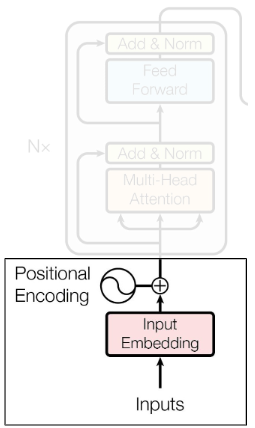
\includegraphics[width=0.5\paperwidth,height=0.5\paperheight,keepaspectratio]{images/introduction-to-transformers/transformer_input_embedding_block_diagram.png}

      {\scriptsize Source: CMU 11-785, Lecture 19, Spring 2024.}
    \end{column}
  \end{columns}
\end{frame}

\begin{frame}{Positional Encodings}
  \centering
  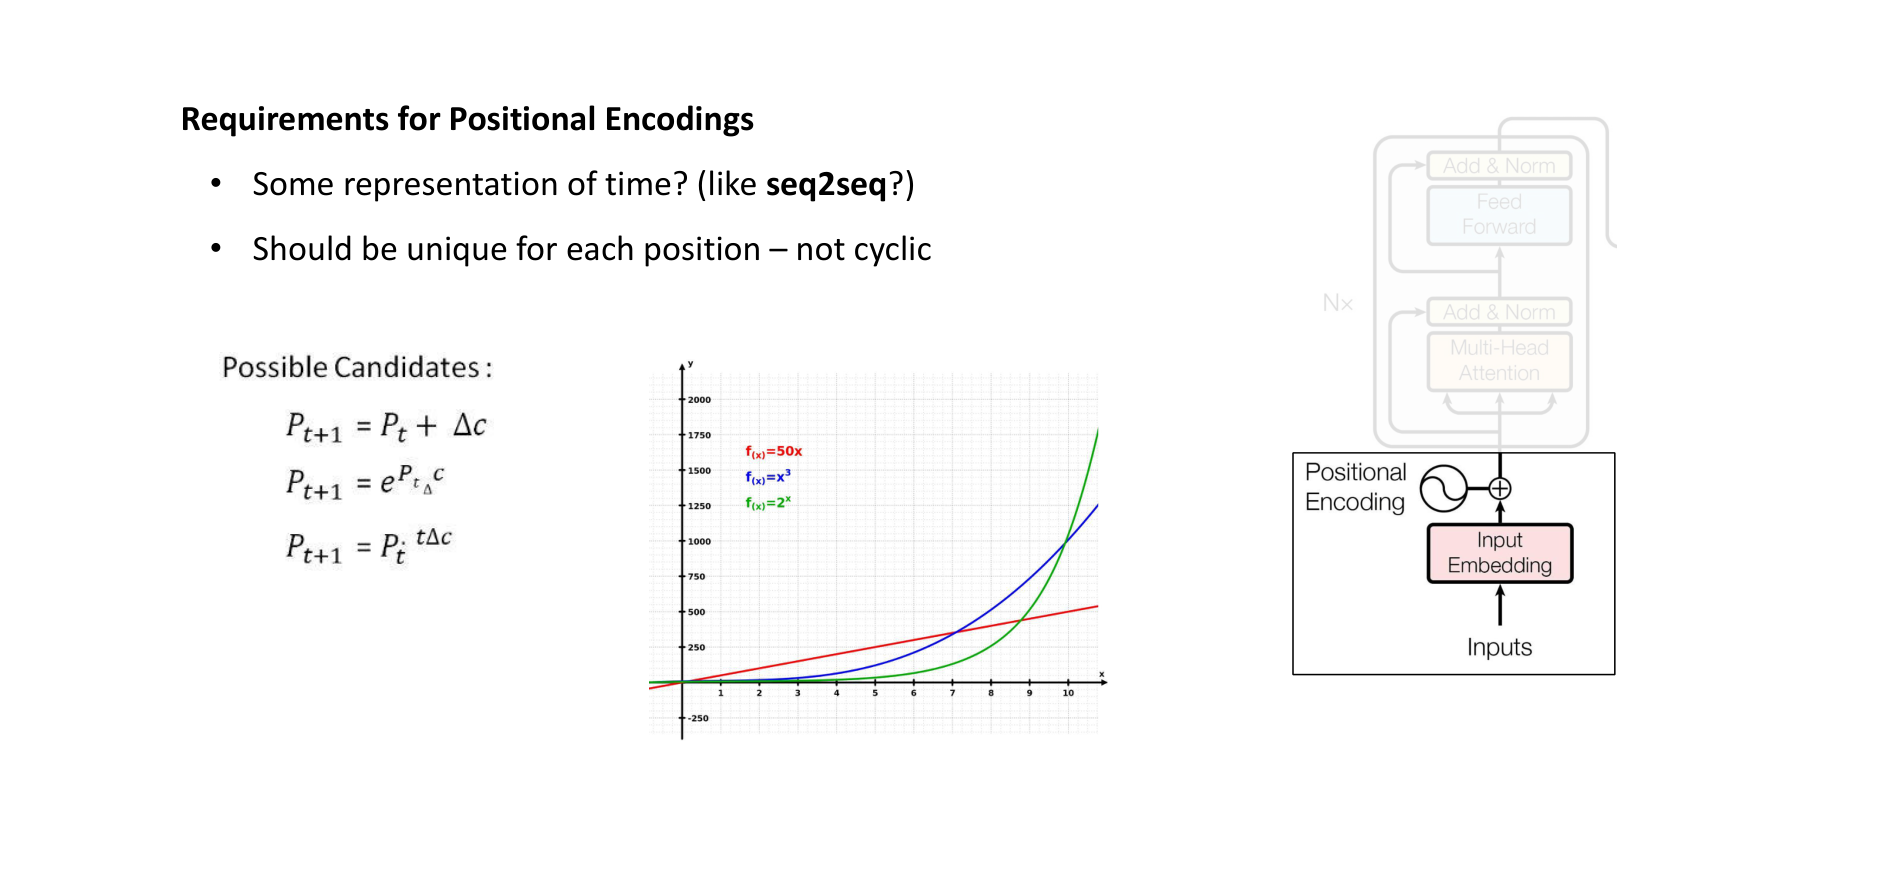
\includegraphics[width=\linewidth,height=0.75\paperheight,keepaspectratio]{images/introduction-to-transformers/transformer_positional_encoding_requirements_candidate_functions.png}

  {\scriptsize Source: CMU 11-785, Lecture 19 ``Transformers,'' Spring 2024, slide 18.}
\end{frame}

\begin{frame}{Positional Encodings}
  \centering
  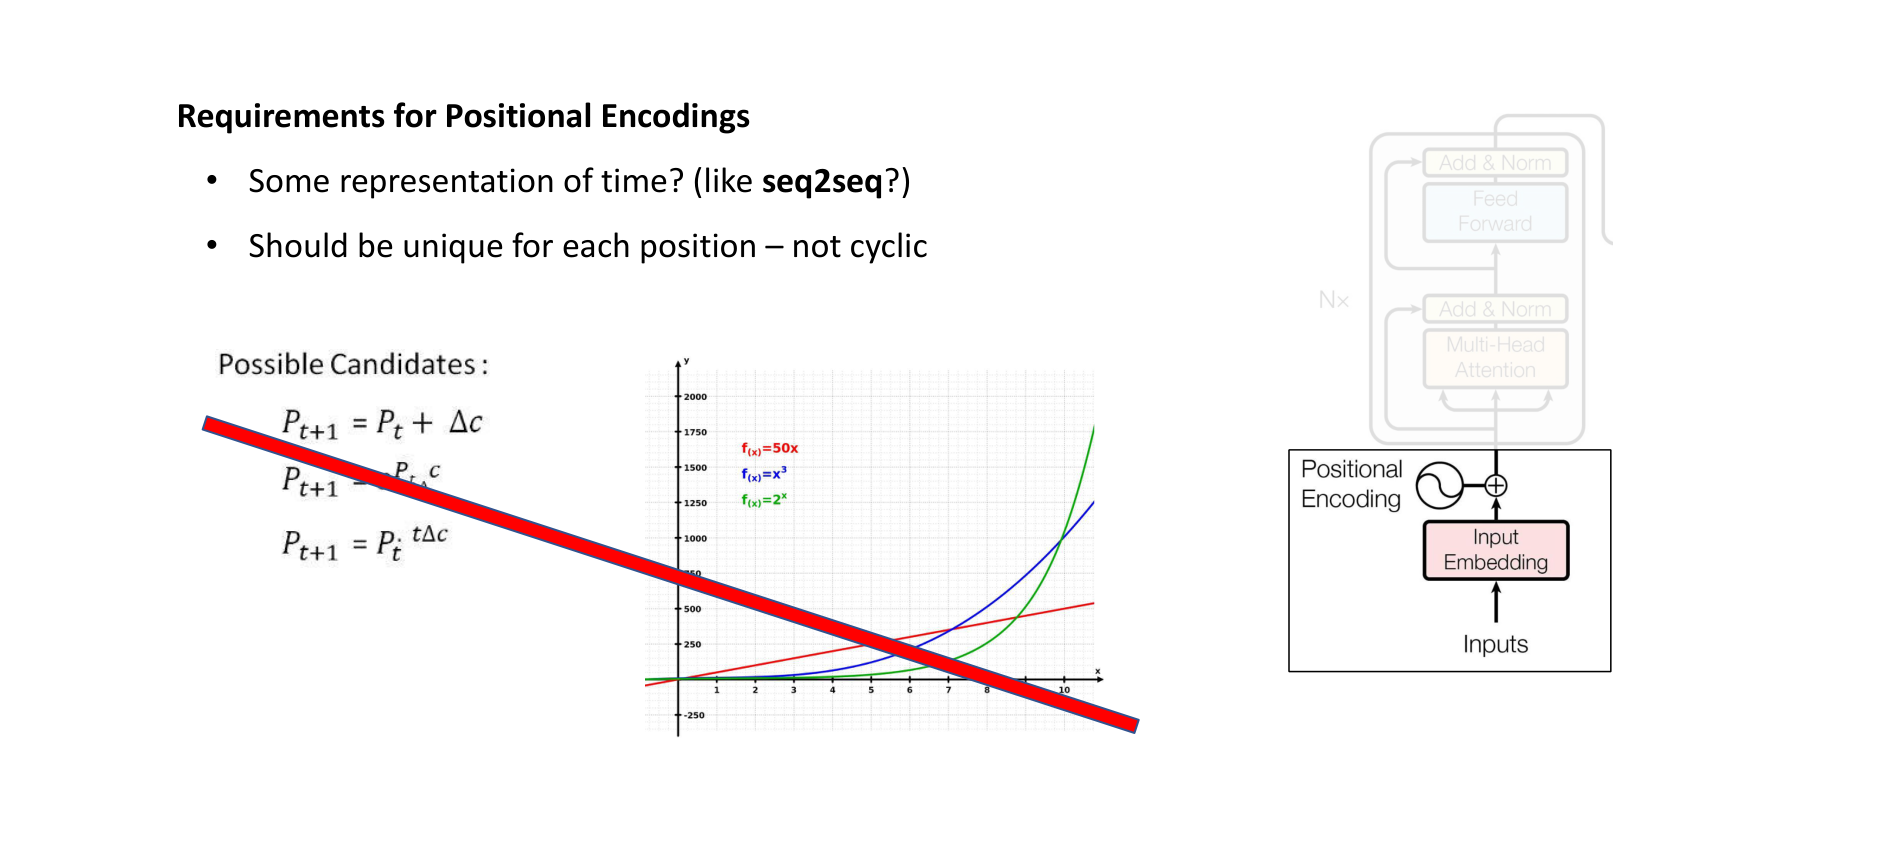
\includegraphics[width=\linewidth,height=0.75\paperheight,keepaspectratio]{images/introduction-to-transformers/transformer_positional_encoding_candidates_rejected.png}

  {\scriptsize Source: CMU 11-785, Lecture 19 ``Transformers,'' Spring 2024, slide 19.}
\end{frame}

\begin{frame}{Position Encodings}
  \begin{columns}
    \begin{column}{0.6\textwidth}
      \textbf{Requirements for Positional Encodings}
      \begin{itemize}
        \item Some representation of time? (like \texttt{seq2seq}?)
        \item Should be unique for each position -- not cyclic
        \item \textbf{Bounded}
      \end{itemize}

      \textbf{Possible Candidates}
      \[
        P(t + t') = M^{t'} \times P(t)
      \]

    \end{column}
    \begin{column}{0.4\textwidth}
      \centering
      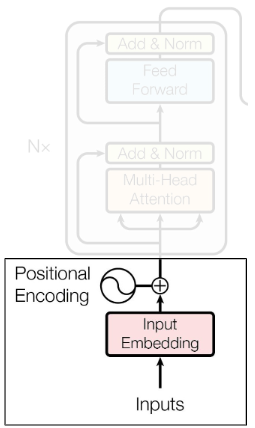
\includegraphics[width=0.5\paperwidth,height=0.5\paperheight,keepaspectratio]{images/introduction-to-transformers/transformer_input_embedding_block_diagram.png}

      {\scriptsize Source: CMU 11-785, Lecture 19, Spring 2024.}
    \end{column}
  \end{columns}
\end{frame}

\begin{frame}{Position Encodings}
  \begin{columns}
    \begin{column}{0.6\textwidth}
      \textbf{Requirements for Positional Encodings}
      \begin{itemize}
        \item Some representation of time? (like \texttt{seq2seq}?)
        \item Should be unique for each position -- not cyclic
        \item \textbf{Bounded}
      \end{itemize}

      \textbf{Possible Candidates}
      \[
        P(t + t') = M^{t'} \times P(t)
      \]

      \vspace{0.8em}
      {\color{blue}\textbf{M?}}
      \begin{enumerate}
        \item Should be a unitary matrix
        \item Magnitudes of eigenvalues should be 1 $\,\rightarrow\,$ norm preserving
        \item The matrix can be learnt
        \item Produces unique rotated embeddings each time
      \end{enumerate}
 

    \end{column}
    \begin{column}{0.4\textwidth}
      \centering
      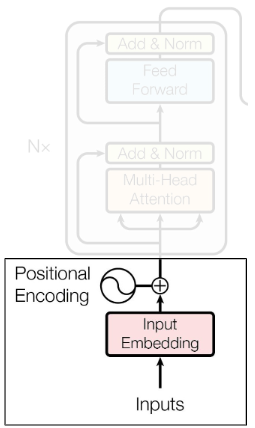
\includegraphics[width=0.5\paperwidth,height=0.5\paperheight,keepaspectratio]{images/introduction-to-transformers/transformer_input_embedding_block_diagram.png}

      {\scriptsize Source: CMU 11-785, Lecture 19, Spring 2024.}
    \end{column}
  \end{columns}
\end{frame}

\begin{frame}{Positional Encodings}
  \centering
  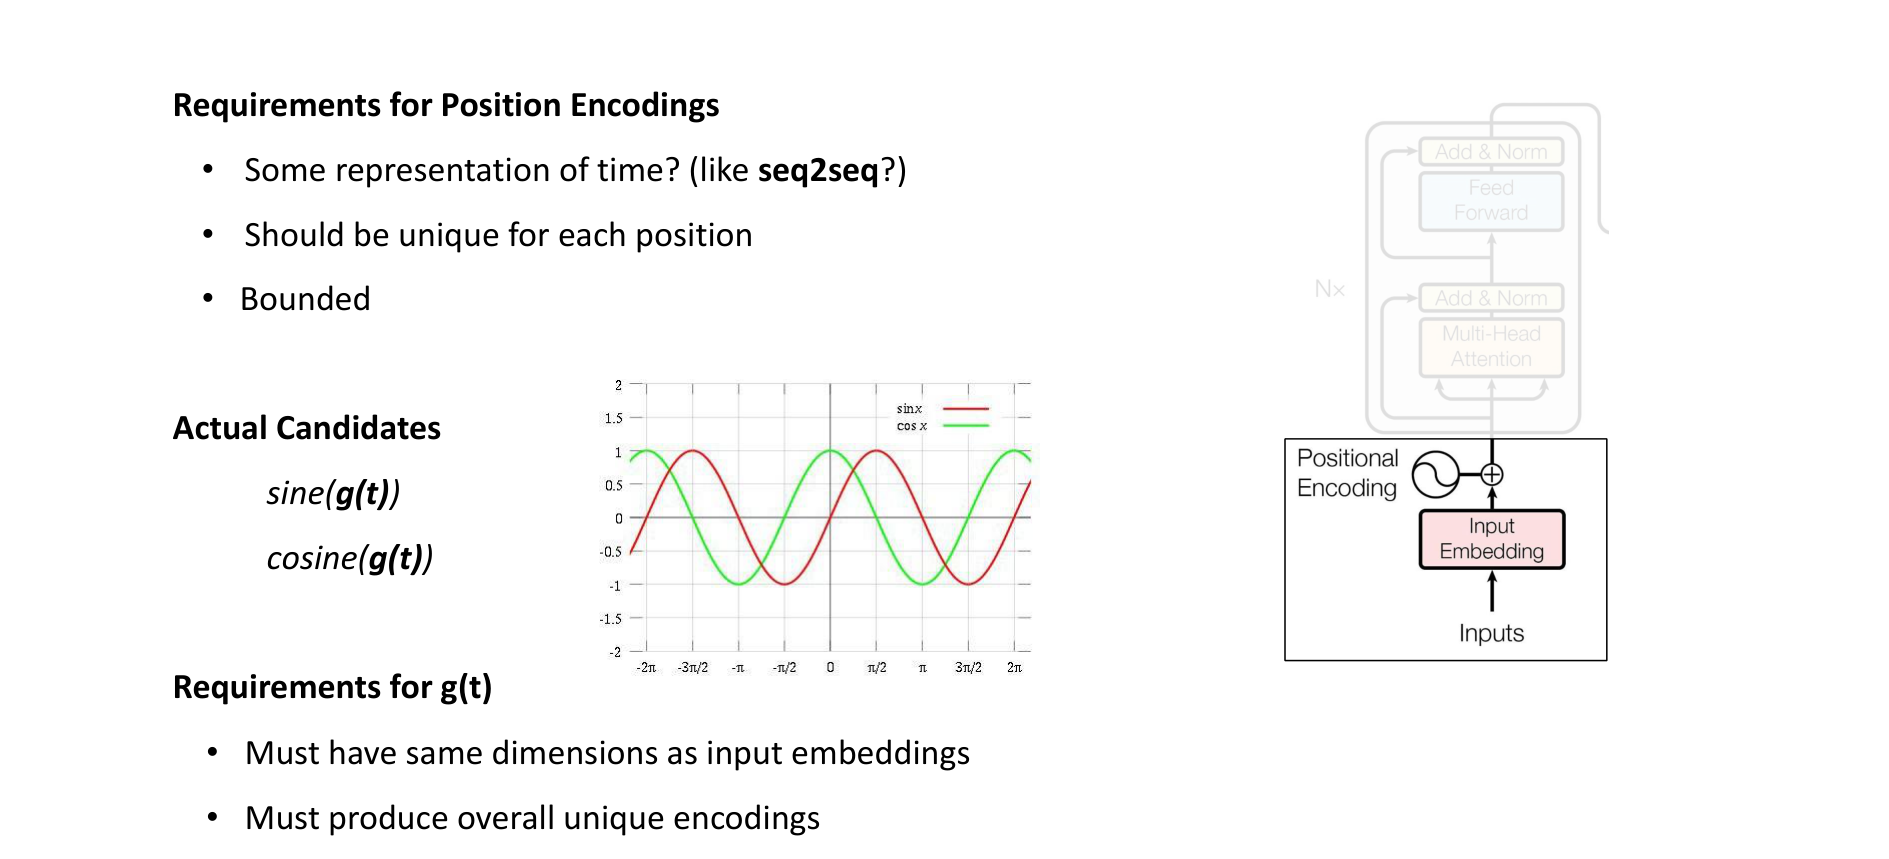
\includegraphics[width=\linewidth,height=0.75\paperheight,keepaspectratio]{images/introduction-to-transformers/transformer_positional_encoding_sine_cosine_candidates.png}

  {\scriptsize Source: CMU 11-785, Lecture 19 ``Transformers,'' Spring 2024, slide 23.}
\end{frame}


\begin{frame}{Position Encoding}
  \begin{columns}
    \begin{column}{0.6\textwidth}
      For each position, an embedded input is moved the same distance but at a different angle. \textbf{Inputs that are close to each other in the sequence have similar perturbations, but inputs that are far apart are perturbed in different directions.}

      \[
        PE_{(pos,\,2i)} = \sin\left( pos / 10000^{2i/d_{\text{model}}} \right)
      \]
      \[
        PE_{(pos,\,2i+1)} = \cos\left( pos / 10000^{2i/d_{\text{model}}} \right)
      \]

      \vspace{0.5em}
      \begin{description}
        \item[pos] idx of the token in input sentence
        \item[i] $i^\text{th}$ dimension out of $d_\text{model}$
        \item[$d_\text{model}$] embedding dimension of each token
      \end{description}
      Different calculations for odd and even embedding indices.

      {\footnotesize Each dimension is periodic; the full vector is not.}

    \end{column}
    \begin{column}{0.4\textwidth}
      \centering
      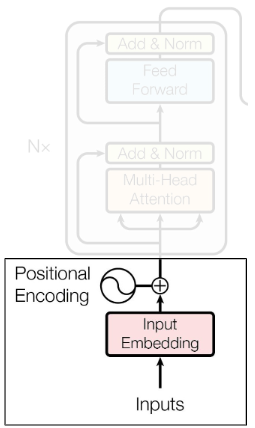
\includegraphics[width=0.5\paperwidth,height=0.5\paperheight,keepaspectratio]{images/introduction-to-transformers/transformer_input_embedding_block_diagram.png}

      {\scriptsize Source: CMU 11-785, Lecture 19, Spring 2024.}
    \end{column}
  \end{columns}
\end{frame}

\begin{frame}{Position Encoding}
  \centering
  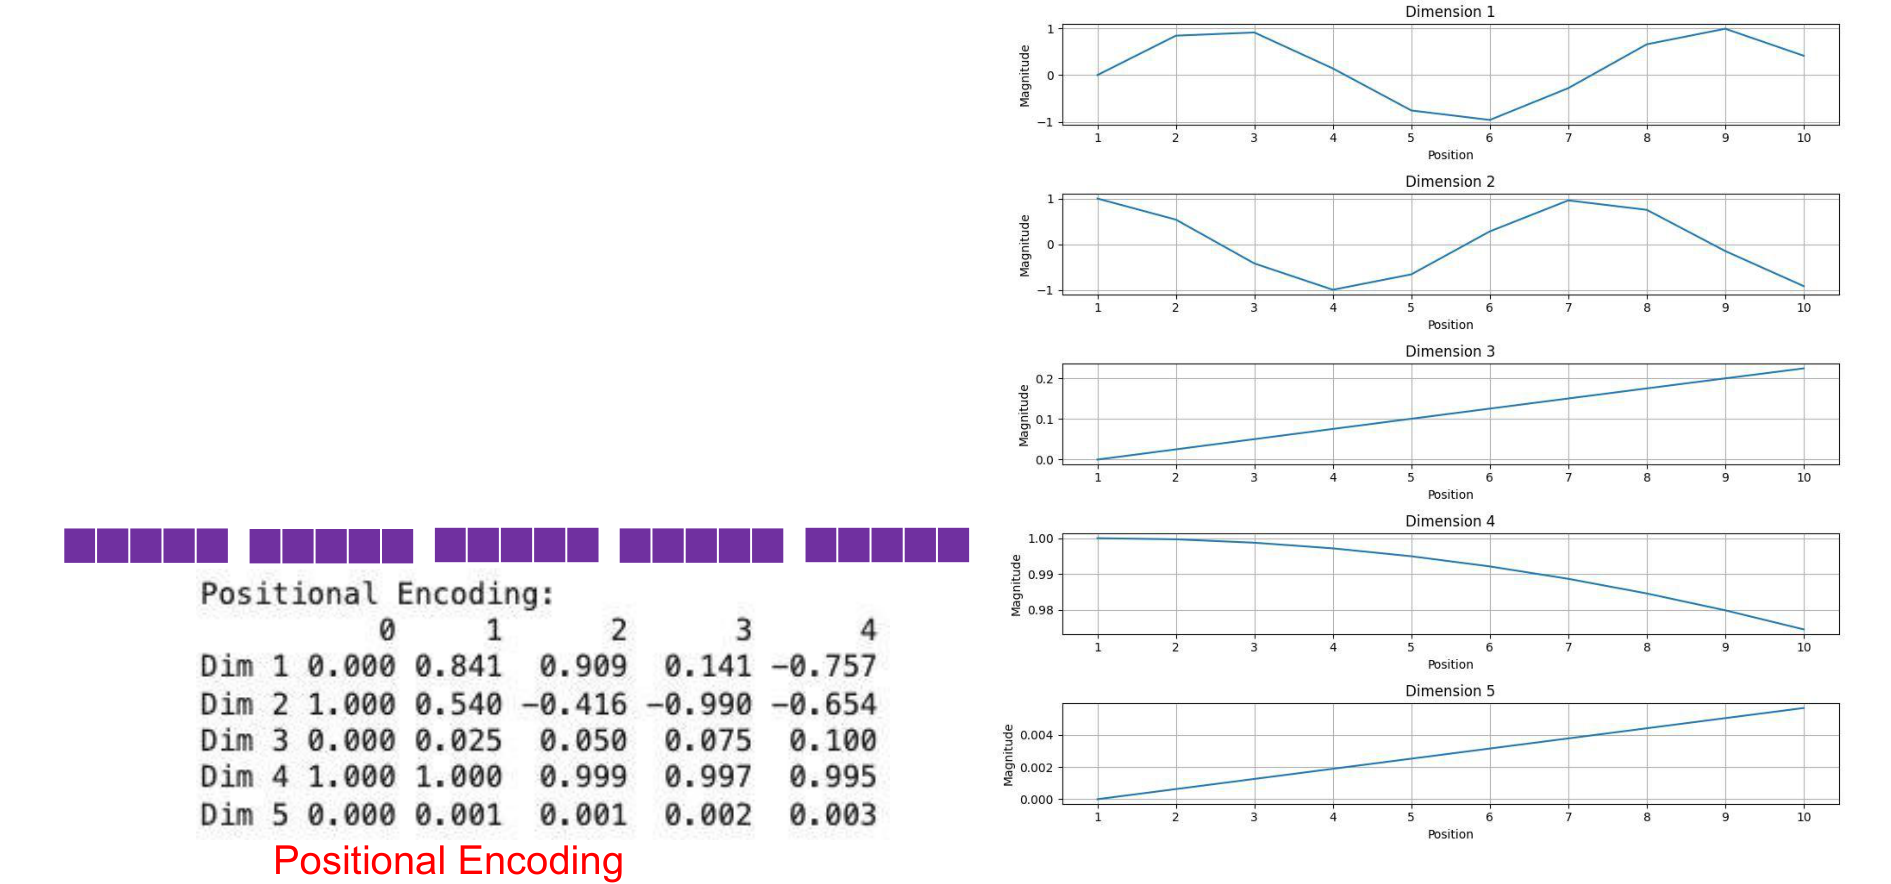
\includegraphics[width=0.8\paperwidth,height=0.75\paperheight,keepaspectratio]{images/introduction-to-transformers/transformer_positional_encoding_matrix_dimension_curves.png}

  {\scriptsize Source: CMU 11-785, Lecture 19 ``Transformers,'' Spring 2024, slide 25.}
\end{frame}

\begin{frame}{Position Encoding}
  \centering
  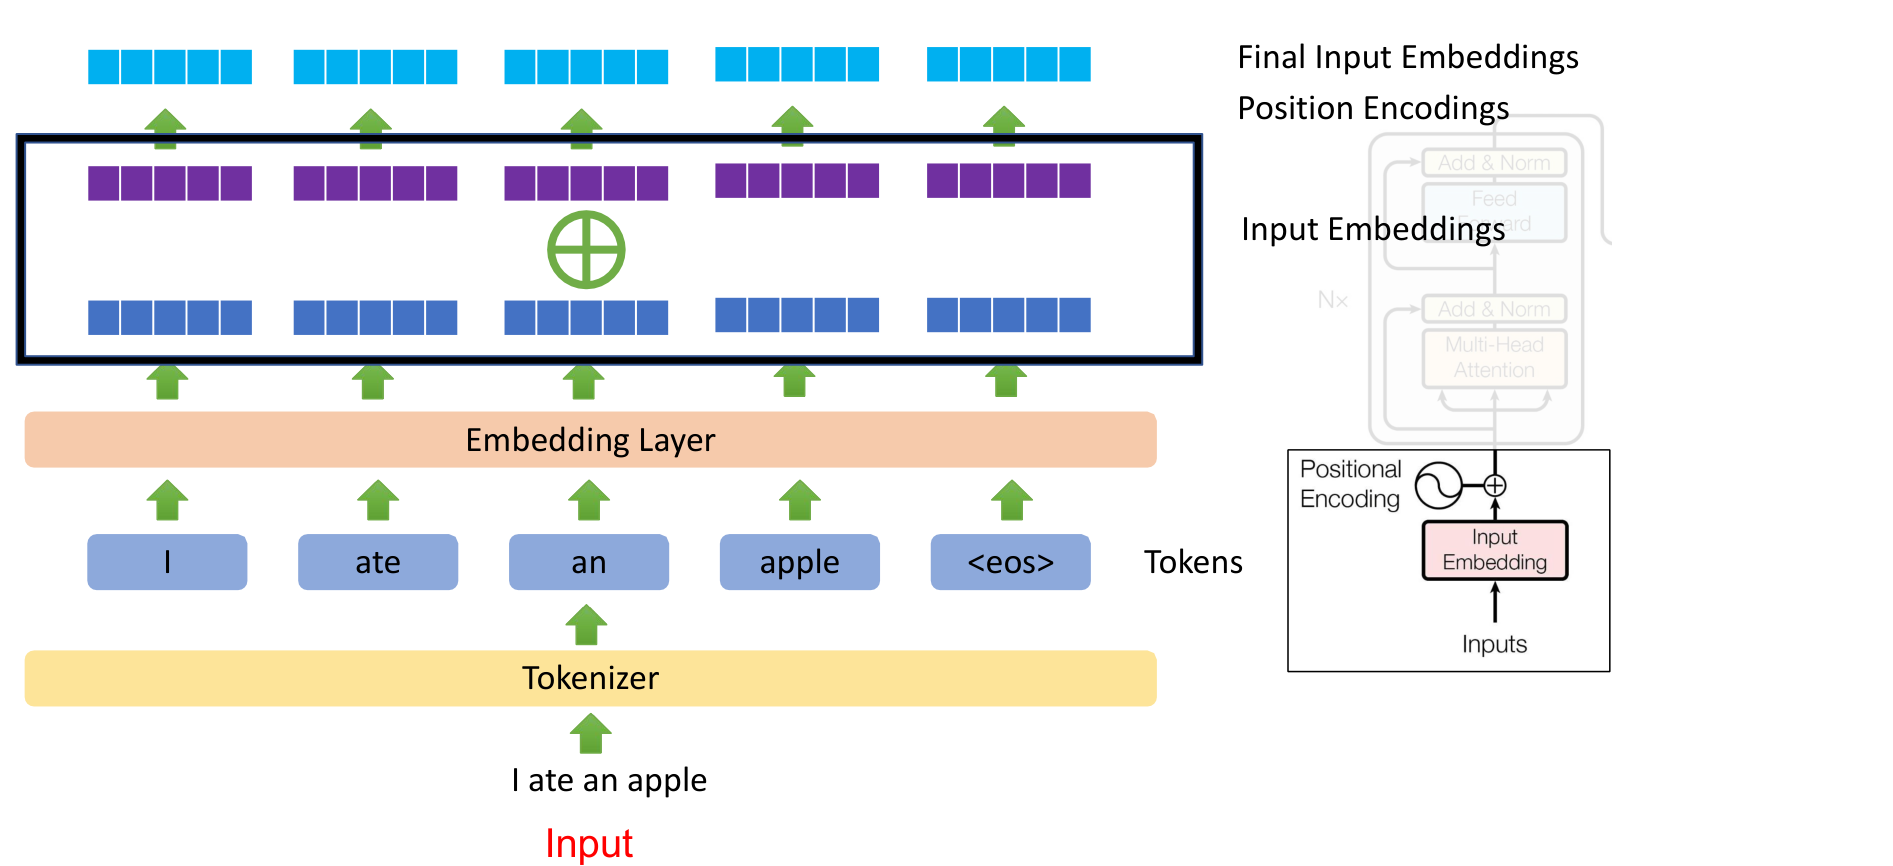
\includegraphics[width=0.8\paperwidth,height=0.75\paperheight,keepaspectratio]{images/introduction-to-transformers/transformer_final_input_embeddings_tokenizer_pipeline.png}

  {\scriptsize Source: CMU 11-785, Lecture 19 ``Transformers,'' Spring 2024, slide 26.}
\end{frame}

\begin{frame}{Alternatives to Positional Encoding}
  \begin{itemize}
    \item[\textcolor{red}{$\blacktriangleright$}] \textbf{Learnable position embeddings:}
    \begin{itemize}
      \item Position embeddings are parameters learned during training.
      \item Allow the model to adapt position representations to the task.
    \end{itemize}
    \vspace{0.5em}
    \item[\textcolor{red}{$\blacktriangleright$}] \textbf{Rotary Position Embeddings (RoPE):}
    \begin{itemize}
      \item Encodes positions by rotating query and key vectors in multi-head attention.
      \item Enables better extrapolation to longer sequences.
    \end{itemize}
    \vspace{0.5em}
    \item[\textcolor{red}{$\blacktriangleright$}] \textbf{ALiBi (Attention with Linear Biases):}
    \begin{itemize}
      \item Adds linear biases to attention scores based on distance between tokens.
      \item Encourages attention to nearby tokens without explicit position embeddings.
    \end{itemize}
  \end{itemize}
\end{frame}

